\begin{figure}
  \centering

  \begin{subfigure}[t]{\textwidth}
    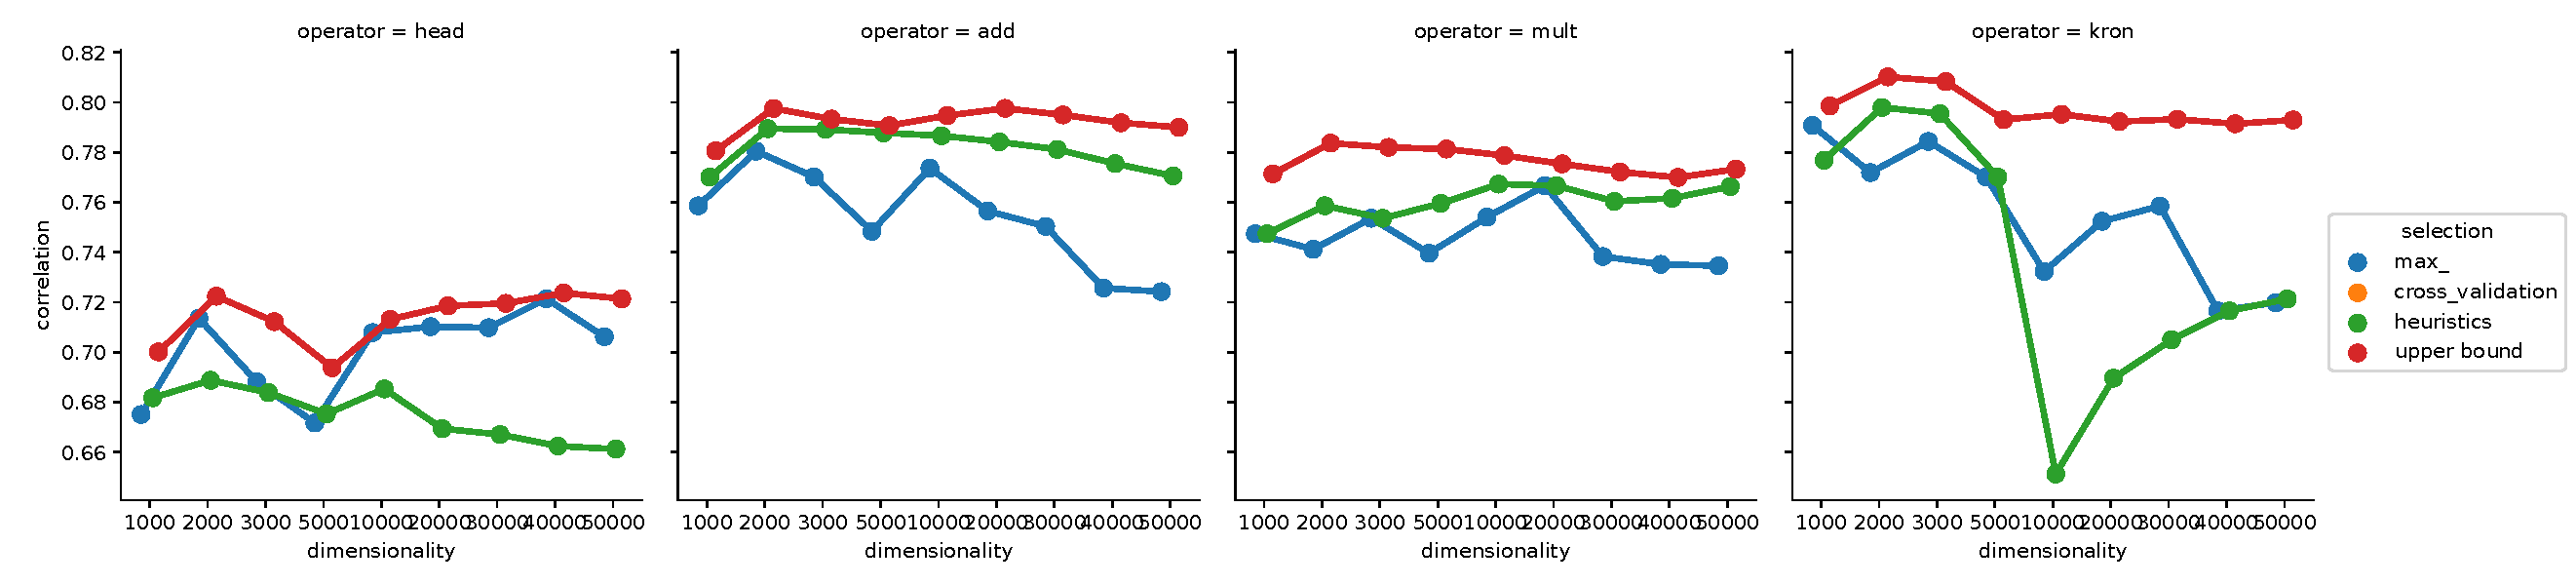
\includegraphics[width=\textwidth]{supplement/figures/compositional-results-ks14}
    \caption{KS14.}
    \label{fig:compositional-results-ks14}
  \end{subfigure}

  \begin{subfigure}[t]{\textwidth}
    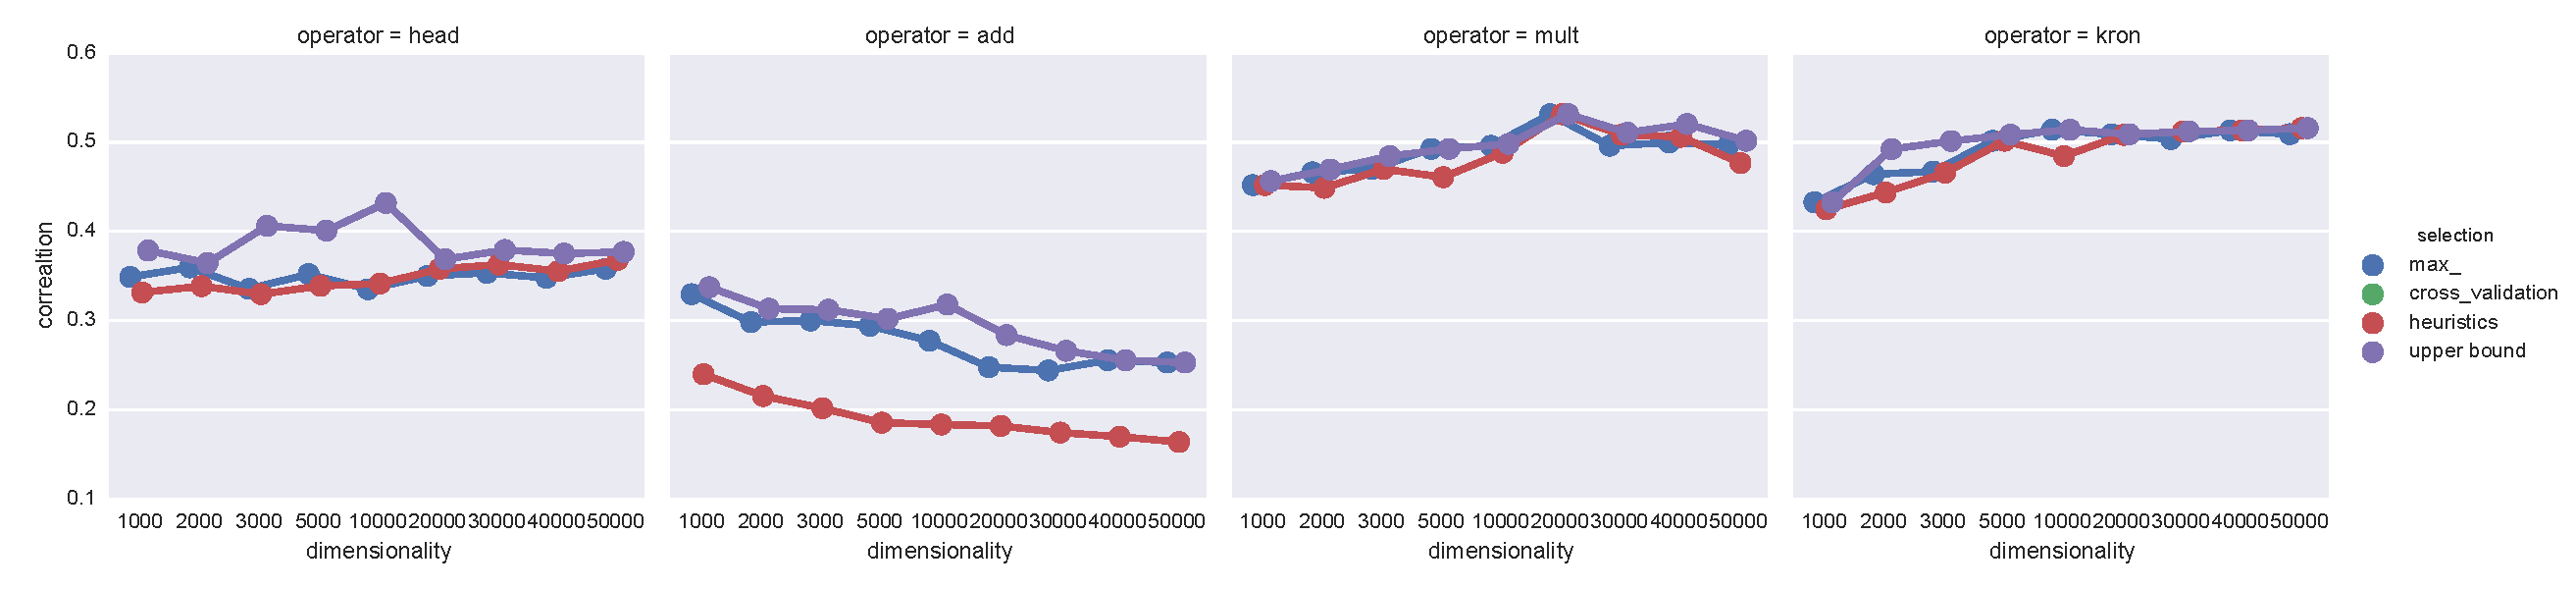
\includegraphics[width=\textwidth]{supplement/figures/compositional-results-gs11}
    \caption{GS11.}
    \label{fig:compositional-results-gs11}
  \end{subfigure}

  \begin{subfigure}[t]{\textwidth}
    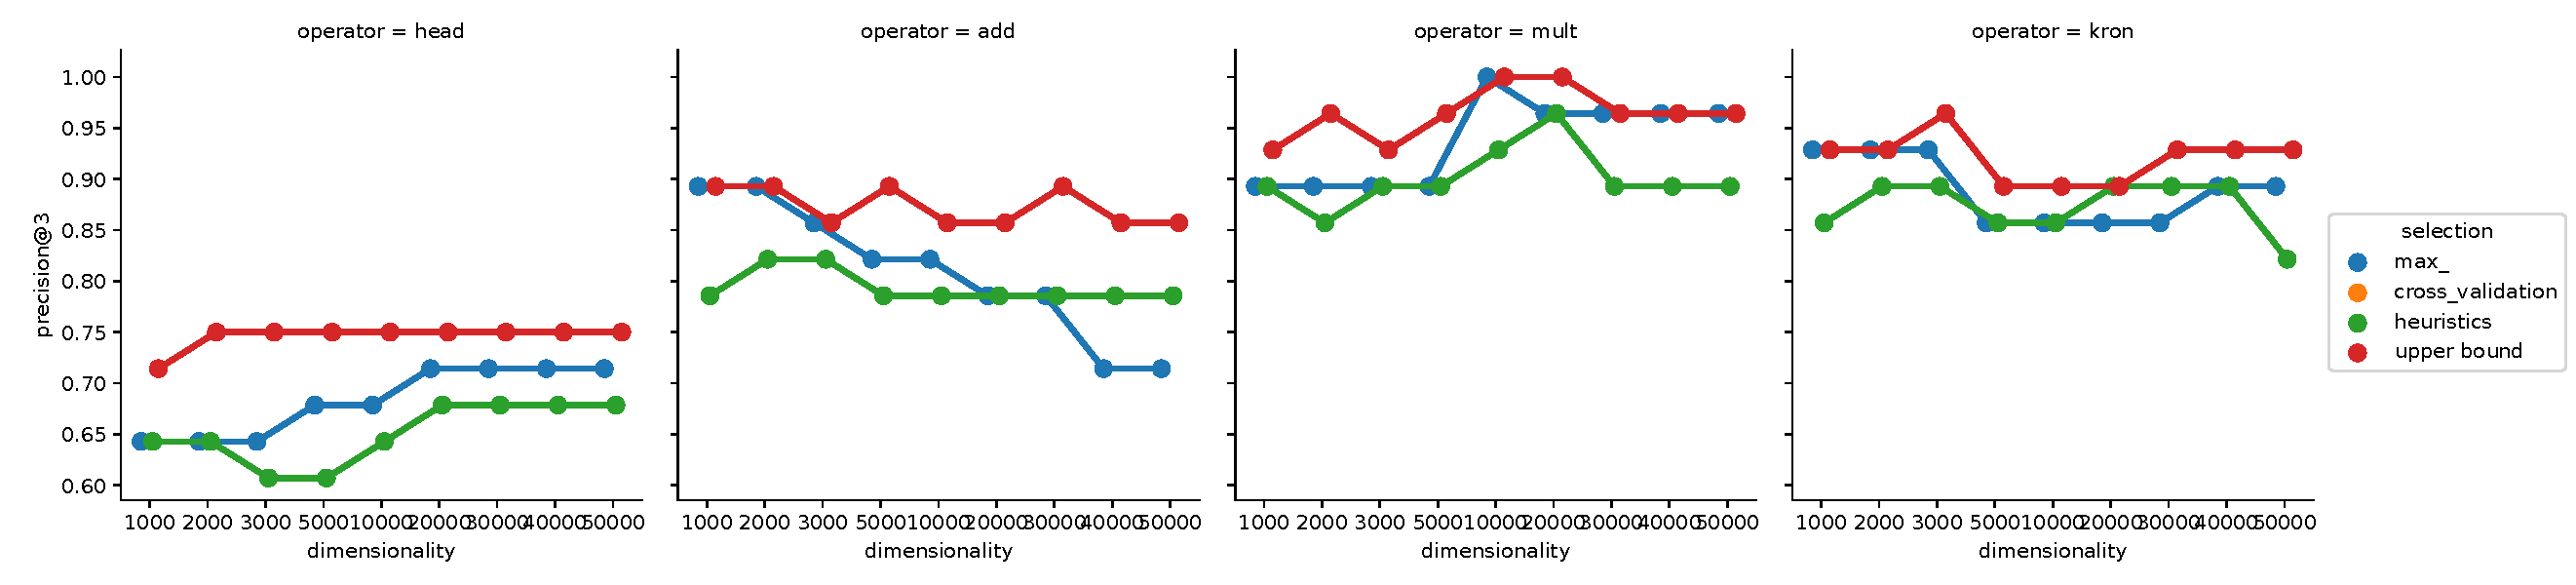
\includegraphics[width=\textwidth]{supplement/figures/compositional-results-phraserel}
    \caption{PhraseRel.}
    \label{fig:compositional-results-phraserel}
  \end{subfigure}


  \caption{Performance of models based on the selection over the average compositional performance}
  \label{fig:compositional-results}
\end{figure}

%%% Local Variables:
%%% mode: latex
%%% TeX-master: "../thesis"
%%% End:
